% !TeX root = er.tex

\chapter{Sensores}\label{ch.sensors}

Um robô não pode mover uma distância específica em uma direção específica apenas ajustando a potência relativa dos motores das duas rodas e o período de tempo em que os motores funcionam. Suponhamos que queiramos que o robô se mova para frente. Se ajustarmos a potência dos dois motores ao mesmo nível, mesmo pequenas diferenças nas características dos motores e rodas farão com que o robô curve ligeiramente para um lado. Desníveis na superfície sobre a qual o robô se move também farão com que as rodas girem em velocidades diferentes. O aumento ou diminuição do atrito entre as rodas e a superfície pode afetar a distância movimentada em um período de tempo específico. Portanto, se quisermos que o robô se mova em direção a uma parede a 1 m de distância e pare 20 cm à sua frente, o robô deve \emph{sentir} a existência da parede e parar quando ele \emph{detectar} que a parede está a 20 cm de distância.

Um \emph{sensor} é um componente que mede alguns aspectos do ambiente. O computador no robô usa tais medidas para controlar as ações do robô. Um dos sensores mais importantes na robótica é o sensor de distância que mede a distância entre o robô e um objeto. Usando vários sensores de distância, ou girando um sensor como esse, o ângulo do objeto em relação à frente do robô pode ser medido. Sensores de distância baratos usando luz infravermelha ou ultrassom são invariavelmente usados em robôs educacionais; robôs industriais frequentemente usam sensores a laser caros porque eles são altamente precisos.

Som e luz também são usados para \emph{comunicação} entre dois robôs, como descrito no Cap.~\ref{ch.swarm}.

Um conhecimento mais amplo do ambiente pode ser obtido através da análise de imagens tiradas por uma câmera. Embora as câmeras sejam muito pequenas e baratas (cada smartphone tem uma), a quantidade de dados em uma imagem é muito grande e os algoritmos de processamento de imagem requerem recursos computacionais significativos. Portanto, as câmeras são usadas principalmente em aplicações complexas, como veículos autônomos.

A seção~\ref{s.classify} introduz a terminologia dos sensores. A seção~\ref{s.distance-sensors} apresenta os sensores de distância, os sensores mais usados por robôs educacionais. Na sequência, a seção ~\ref{s.cameras} trata sobre câmeras e, em seguida, uma breve discussão sobre outros sensores que os robôs usam é apresentada (seção~\ref{s.other-sensors}). A seção ~\ref{s.range} define as características dos sensores: alcance, resolução, precisão, precisão. O capítulo é concluído com uma discussão sobre a não-linearidade dos sensores (Sect.~\ref{s.nonlinearity}).


\section{Classificação dos Sensores}\label{s.classify}

Sensores são classificados como \emph{proprioceptivos} ou \emph{exteroceptivos}, estes posteriormente divididos em \emph{ativos} e \emph{passivos} (Fig.~\ref{fig.sensor-classification}). Um sensor proprioceptivo mede algo interno ao próprio robô. Um exemplo familiar é um velocímetro de um carro, que mede a velocidade do próprio veículo através da contagem das rotações de suas rodas (Sect.~\ref{s.wheel}). Um sensor exteroceptivo mede algo externo ao robô, como sua distância a um objeto. Um sensor ativo afeta o ambiente normalmente através da emissão de energia: um \emph{sonar} de um submarino emite ondas sonoras e usa sua reflexão para determinar a distância a obstáculos. Já um sensor passivo não afeta o ambiente: uma câmera simplesmente detecta a luz refletida por objetos presentes na cena. Robôs invariavelmente utilizam algum sensor exteroceptivo para lidar com erros que possam surgir por causa de sensores proprioceptivos ou para considerar alterações no ambiente. 

\begin{figure}
\begin{center}
\begin{tikzpicture}[node distance = 4mm and 1cm]
\node (sensor) { \textsf{sensor} };
\node (ex) [above right=of sensor] { \textsf{exteroceptivo} };
\node (pro) [below right=of sensor] { \textsf{proprioceptivo} };
\node (active) [above right=of ex] { \textsf{ativo} };
\node (passive) [below right=of ex] { \textsf{passivo} };
\draw (sensor) -- (pro);
\draw (sensor) -- (ex);
\draw (ex) -- (active);
\draw (ex) -- (passive);
\end{tikzpicture}
\caption{Classificação dos sensores}\label{fig.sensor-classification}
\end{center}
\end{figure}

\section{Sensor de Distância}\label{s.distance-sensors}

Na maioria das aplicações, o robô precisa medir sua distância a um objeto usando um sensor de distância. Os sensores de distância são normalmente \emph{ativos}: eles transmitem um sinal e depois recebem sua reflexão (se houver) de um objeto (Fig.~\ref{fig.measure-d}). Uma maneira de determinar a distância é medir o tempo que decorre entre o envio de um sinal e a recepção de sua reflexão:
\begin{equation}
s = \frac{1}{2}vt\,,\label{eq.reflected}
\end{equation}
onde $s$ é a distância, $v$ é a velocidade do sinal e $t$ é o tempo decorrido entre o envio e a recepção do sinal refletido. A divisão por dois se deve ao fato de que o sinal percorre a distância duas vezes: do robô para o objeto e de volta após sua reflexão. Outra maneira de calcular a distância é usando a técnica de triangulação, explicada na seção.~\ref{s.triangulating-sensors}.

\begin{figure}
\begin{center}
\begin{tikzpicture}
\draw[xshift=-1mm] pic { robot };
\foreach \x in {14, 18, 22, 26, 30, 34}
\draw[blue] (\x mm,-10mm) arc[start angle=-30, end angle=30, radius=20mm];
\draw[fill] (38mm,0) circle[radius=3pt];
\foreach \x in {16, 20, 24, 28, 32, 36}
\draw[thick,dashed,red] (\x mm,-10mm) arc[start angle=210, end angle=150, radius=20mm];
\end{tikzpicture}
\end{center}
\caption{Medindo a distância através da transmissão de uma onda e recebimento de sua reflexão}\label{fig.measure-d}
\end{figure}

Os sensores de distância de baixo custo são baseados em outro princípio: como a intensidade de um sinal diminui com a distância, medir a intensidade de um sinal refletido dá uma indicação da distância do sensor a um objeto. A desvantagem desse método é que a intensidade do sinal recebido é influenciada por fatores tais como a refletividade do objeto.

\subsection{Sensores de Distância por Ultrassom}

O ultrassom é som cuja frequência está acima de $20,\!000$ hertz, maior do que a frequência mais alta que pode ser ouvida pelo ouvido humano. Há dois ambientes em que o som é melhor que a visão: à noite e na água. Os morcegos usam o ultrassom para navegar quando voam à noite porque depois do pôr-do-sol há pouca luz natural para a localização de alimentos. Navios e submarinos usam o ultrassom para detectar objetos porque o som viaja muito melhor na água do que no ar. Verifique você mesmo, indo dar um mergulho em um lago lamacento ou no oceano: a que distância você pode ver um amigo? Agora, peça-lhe para fazer um som batendo dois objetos juntos ou batendo palmas. A que distância você pode ouvir o som? 

A velocidade do som no ar é de cerca de $340$ m/s ou $34,\!000$ cm/s. Se um objeto está a uma distância de $34$ cm de um robô, da Eq.~\ref{eq.reflected} segue-se que um sinal de ultrassom viajará até o objeto e será refletido de volta em:
\[\frac{2\cdot 34}{34000} = \frac{2}{1000} = 2\times 10^{-3}\  \textrm{segundos} = 2\  \textrm{milissegundos}.\]
Um circuito eletrônico pode medir facilmente períodos de tempo da ordem de milissegundos.

A vantagem dos sensores de ultrassom é que eles não são sensíveis a mudanças na cor ou refletividade da luz dos objetos, nem à intensidade da luz no ambiente. Eles são, no entanto, sensíveis à textura: o tecido absorverá parte do som, enquanto a madeira ou metal refletirá quase todo o som. É por isso que cortinas, tapetes e objetos macios são usados para tornar os ambientes mais confortáveis.

Os sensores de ultrassom são relativamente baratos e podem funcionar em ambientes externos. Eles são usados em carros para detectar distâncias curtas, como para auxiliar no estacionamento. Sua principal desvantagem é que a medição da distância é relativamente lenta, já que a velocidade do som é muito menor do que a velocidade da luz. Outra desvantagem é que eles não podem ser focalizados a fim de medir a distância até um objeto específico.

\subsection{Sensores de Proximidade Infravermelhos}

\emph{Luz infravermelha} é a luz cujo comprimento de onda é maior que a luz vermelha, que é a luz com o comprimento de onda mais longo que nossos olhos podem ver. O olho pode ver a luz com comprimentos de onda de cerca de $390$ a $700$ nanômetros (um nanômetro é um milionésimo de um milímetro). A luz infravermelha tem comprimento de onda entre $700$ e $1000$ nanômetros. Ela é invisível ao olho humano e, portanto, é usada no controle remoto de aparelhos de TV e outros aparelhos eletrônicos.

Os sensores de proximidade são dispositivos simples que utilizam a luz para detectar a presença de um objeto através da medição da intensidade da luz refletida. A intensidade da luz diminui com o quadrado da distância da fonte e esta relação pode ser usada para medir a distância aproximada ao objeto. A medição da distância não é muito precisa porque a intensidade refletida também depende da refletividade do objeto. Um objeto preto reflete menos luz do que um objeto branco colocado à mesma distância, portanto um sensor de proximidade não pode distinguir entre um objeto preto próximo e um objeto branco colocado um pouco mais distante. Esta é a razão pela qual esses sensores são chamados sensores de proximidade, não sensores de distância. A maioria dos robôs educacionais usa sensores de proximidade porque são muito mais baratos do que os sensores de distância.

\subsection{Sensores Ópticos de Distância}\label{s.optical-distance}

A distância pode ser calculada a partir de uma medida do tempo decorrido entre o envio de um sinal luminoso e a recepção de sua reflexão. A luz pode ser luz comum ou luz de um laser. A luz produzida por um laser é \emph{coerente} (ver abaixo).  Mais comumente, os lasers para medir distância usam luz infravermelha, embora a luz visível também possa ser usada. Os lasers têm várias vantagens em relação a outras fontes de luz. Primeiro, os lasers são mais potentes e podem detectar e medir distância a objetos mais longínquos. Em segundo lugar, um feixe laser é altamente focalizado, o que permite que uma medição precisa do ângulo até o objeto seja feita (Fig.~\ref{fig.beam}).

\begin{figure}
\begin{center}
\begin{tikzpicture}
\draw pic { robot };
\draw[fill] (20:5) circle[radius=3pt];
\draw[blue] (0,0) -- (17:5) arc[start angle=17, end angle=23, radius=5cm] -- cycle;
\draw[dashed,red] (0,0) -- (10:5) arc[start angle=10, end angle=30, radius=5cm] -- cycle;
\end{tikzpicture}
\end{center}
\caption{Largura do feixe de luz laser (sólido) e luz não-coerente (tracejado)}\label{fig.beam}
\end{figure}

\begin{quote}
\begin{center}
\textbf{Luz coerente}
\end{center}
Três tipos de luz são mostrados na Fig.~\ref{fig.coherent}. A luz do sol ou de uma lâmpada incandescente é chamada \emph{luz branca} porque é composta de luz de muitas cores diferentes (frequências), emitida em diferentes momentos (fases) e emitida em diferentes direções. Os diodos emissores de luz (LED) emitem \emph{luz monocromática} (luz de uma única cor), mas não são coerentes porque suas fases são diferentes e sua luz é emitida em diferentes direções. Os lasers emitem \emph{luz coerente}: todas as ondas são da mesma frequência e estão em fase (o início de cada onda é ao mesmo tempo). Toda a energia é concentrada em um feixe estreito e a distância pode ser calculada medindo seu tempo de voo (da emissão à detecção do sinal refletido) ou a diferença de fase da luz refletida.
\end{quote}

\begin{figure}
\begin{center}
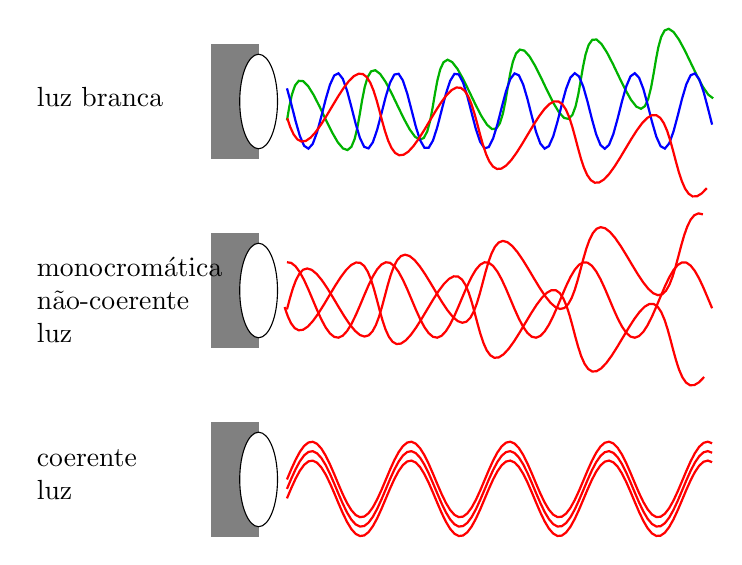
\begin{tikzpicture}[scale=.6,domain=0:9,align=left]
\draw[fill,gray] (-16mm,-8mm) rectangle +(10mm,24mm);
\draw[fill=white] (-6mm,4mm) circle[x radius=4mm, y radius=10mm];
\node[anchor=west] at (-5.5,5mm) {\p{luz branca}};
\draw[samples=100,green!70!black,thick,rotate=8] plot (\x,{.8*sin(4*\x r)});
\draw[samples=100,blue,thick,yshift=2mm] plot (\x,{.8*sin(5*(\x+.5) r)});
\draw[samples=100,red,thick,rotate=-8,yshift=4mm] plot (\x,{.8*sin(3*(\x+1.2) r)});
\begin{scope}[yshift=-4cm]
\draw[fill,gray] (-16mm,-8mm) rectangle +(10mm,24mm);
\draw[fill=white] (-6mm,4mm) circle[x radius=4mm, y radius=10mm];
\node[anchor=west] at (-5.5,2mm) {\p{monocromática}\\\p{não-coerente}\\\p{luz}};
\draw[samples=100,red,thick,rotate=8] plot (\x,{.8*sin(3*\x r)});
\draw[samples=100,red,thick,yshift=2mm] plot (\x,{.8*sin(3*(\x+.5) r)});
\draw[samples=100,red,thick,yshift=4mm,rotate=-8] plot (\x,{.8*sin(3*(\x+1.2) r)});
\end{scope}
\begin{scope}[yshift=-8cm]
\draw[fill,gray] (-16mm,-8mm) rectangle +(10mm,24mm);
\draw[fill=white] (-6mm,4mm) circle[x radius=4mm, y radius=10mm];
\node[anchor=west] at (-5.5,5mm) {\p{coerente}\\\p{luz}};
\draw[samples=100,red,thick] plot (\x,{.8*sin(3*\x r)});
\draw[samples=100,red,thick,yshift=2mm] plot (\x,{.8*sin(3*\x r)});
\draw[samples=100,red,thick,yshift=4mm] plot (\x,{.8*sin(3*\x r)});
\end{scope}
\end{tikzpicture}
\end{center}
\caption{Luz branca, monocromática não-coerente, e coerente}\label{fig.coherent}
\end{figure}

Suponha que um pulso de luz seja transmitido pelo robô, refletido em um objeto e recebido por um sensor no robô. A velocidade da luz no ar é cerca de $300,\!000,\!000$ m/s, que é de $3\times 10^{8}$ m/s ou $3\times 10^{10}$ cm/s em notação científica. Se um sinal luminoso for dirigido a um objeto a $30$ cm do robô, o tempo de transmissão e recepção do sinal é (Fig.~\ref{fig.ir}):
\[\frac{2\cdot 30}{3\times 10^{10}} = \frac{2}{10^{9}} = 2\times 10^{-9}\  \textrm{segundos} = 0,\!002\  \textrm{milissegundos}.\]
Este é um período de tempo muito curto, mas pode ser medido por circuitos eletrônicos.

\begin{figure}
\includegraphics[width=.6\textwidth]{time-of-flight}
\caption{Um sensor de distância de tempo de voo (preto) montado em um circuito impresso de 1,6 mm de espessura (verde).}\label{fig.ir}
\end{figure}

O segundo princípio de medição de distância por um feixe de luz é a triangulação. Nesse caso, o transmissor e o receptor são colocados em locais diferentes. O receptor detecta o feixe refletido em uma posição que é função da distância do objeto em relação ao sensor.

\subsection{Sensores por Triangulação}\label{s.triangulating-sensors}

Antes de explicar como funciona um \emph{sensor por triangulação}, temos de entender como o reflexo da luz depende do objeto em que ela atinge. Quando um feixe de luz estreito como a luz coerente de um laser atinge uma superfície brilhante como um espelho, os raios de luz se refletem também em um feixe estreito. O ângulo de reflexão em relação à superfície do objeto é o mesmo que o ângulo de incidência. Isto é chamado de reflexão \emph{especular} (Fig.~\ref{fig.reflect-left}). Quando a superfície é áspera, a reflexão é \emph{difusa} (Fig.~\ref{fig.reflect-right}), em todas as direções, porque mesmo áreas muito próximas da superfície têm ângulos ligeiramente diferentes. A maioria dos objetos em um ambiente, como pessoas e paredes, refletem difusamente. Portanto, para detectar a luz laser refletida o detector não precisa ser colocado em um ângulo preciso em relação ao transmissor.

\begin{figure}
\begin{minipage}{.45\textwidth}
\begin{tikzpicture}
\draw(5,0) arc[start angle=270, end angle=90, radius=8mm];
\begin{scope}[rotate=-15,xshift=-6mm,yshift=10mm]
\node[draw,rectangle,anchor=west,minimum height=5mm,minimum width=12mm,transform shape] (laser) at (0,8mm) {\p{Laser}};
\node[draw,rectangle,node distance=-.4pt,minimum height=2mm,minimum width=4mm,transform shape] (tip) [right=of laser] {};
\end{scope}
\draw(tip.east) -- ++(-15:28.5mm) -- +(195:30mm);
\end{tikzpicture}
\caption{Reflexão especular\label{fig.reflect-left}}
\end{minipage}
\hspace{\fill}
\begin{minipage}{.45\textwidth}
\begin{tikzpicture}
\draw(5,0) arc[start angle=270, end angle=90, radius=8mm];
\begin{scope}[rotate=-15,xshift=-6mm,yshift=10mm]
\node[draw,rectangle,anchor=west,minimum height=5mm,minimum width=12mm,transform shape] (laser) at (0,8mm) {\p{Laser}};
\node[draw,rectangle,node distance=-.4pt,minimum height=2mm,minimum width=4mm,transform shape] (tip) [right=of laser] {};
\end{scope}
\draw(tip.east) -- ++(-15:28.5mm) coordinate (reflect) -- +(195:10mm);
\foreach \angle in {120,135,150,180,210,225}
  \draw(reflect) -- +(\angle:10mm);
\end{tikzpicture}
\caption{Reflexão difusa\label{fig.reflect-right}}
\end{minipage}
\end{figure}

As figuras~\ref{fig.triangulation-left}--\ref{fig.triangulation-right} mostram um sensor por triangulação simplificado que detecta um objeto a duas distâncias. O sensor consiste de um emissor laser e, a uma distância $d$, uma lente que focaliza a luz recebida em um conjunto de sensores colocados a uma distância de $l$ atrás da lente. Assumindo que o objeto reflete a luz difusa, parte da luz será coletada pela lente e focalizada nos sensores. A distância $d'$ ao longo do conjunto de sensores é inversamente proporcional à distância $s$ do objeto em relação ao emissor laser.

Os triângulos de $d$ e os triângulos de $d'$ são semelhantes, portanto, temos a fórmula:
\[
\frac{s}{d} = \frac{l}{d'}\,.
\]
Como $l$ e $d$ são fixados por construção, medindo $d'$ a partir do índice do sensor que detecta a luz focalizada, podemos calcular $s$, a distância do objeto em relação ao sensor. O sensor tem de ser calibrado medindo a distância $s$ correspondente a cada sensor dentro da matriz, mas uma vez que uma tabela é armazenada dentro do computador, a distância $s$ pode ser obtida através de uma busca de tabela.

Há muitos parâmetros de projeto que afetam o desempenho de um sensor de distância por triangulação: a potência do laser, as características ópticas da lente, o número de sensores na matriz e sua sensibilidade. Além da compensação usual entre desempenho e custo, a principal troca está entre o alcance e a distância mínima na qual um objeto pode ser detectado. Para uma distância $s$ muito curta, o tamanho da matriz do detector $d'$ torna-se muito grande, o que impõe um limite prático para a distância mínima de detecção. Tal distância mínima pode ser reduzida aumentando-se a distância entre o emissor de laser e o conjunto de detectores, mas isto reduz o alcance. Um sensor por triangulação pode ser caracterizado pela distância $s_{\textit{opt}}$ para um ótimo desempenho, a distância mínima e a faixa em torno de $s_{\textit{opt}}$ em que as medições podem ser feitas.

\begin{figure}
\begin{minipage}{.5\textwidth}
\begin{tikzpicture}[scale=.65]
\draw(0,0) rectangle +(3,4);
\node[draw,rectangle,anchor=west,minimum height=5mm,minimum width=12mm] (laser) at (10mm,32mm) {\p{Laser}};
\node[draw,rectangle,node distance=-.4pt,minimum height=2mm,minimum width=2.4mm] (tip) [right=of laser] {};
\draw(26mm,20mm) coordinate (lens) ellipse [x radius=2mm, y radius=4mm];
\draw(28mm,14mm) node {\p{Lente}};
\foreach \y in {8mm,10mm,12mm,14mm,16mm,18mm,20mm,22mm}
  \draw(10mm,\y) circle[radius=1mm];
\draw(13mm,4mm) node {\p{Detectores}};
\node[draw,rectangle,fill,color=lightgray,minimum height=8mm,minimum width=2mm] (object) at (70mm,32mm) {};
\draw(70mm,22mm) node {\p{Objeto}};
% Triangles
\draw[thick,blue] (tip.east) -- node[right,black] {$d$} (lens.center);
\draw[thick,green!60!black,densely dashed] (lens.center) -- node[above,black] {$l$} +(-16mm,0) coordinate (sensor);
\draw[blue,thick] (sensor) -- node[left,black] {$d'$} ($ (object.west) ! 1.373 ! (lens.center) $) coordinate (sensor1);
\draw[densely dashed,thick,green!60!black] (tip.east) -- node[above,black] {$s$} (object.west);
\draw[red,thick] (object.west) -- ($ (object.west) ! 1.373 ! (lens.center) $) coordinate (sensor1);
\fill(tip.east) circle[radius=.8pt];
\fill(lens.center) circle[radius=.8pt];
\fill(sensor) circle[radius=.8pt];
\fill(sensor1) circle[radius=.8pt];
\node at (48mm,22mm) {$s'$};
\node at (18mm,14mm) {$l'$};
\end{tikzpicture}
\caption{Triangulação de um objeto distante}\label{fig.triangulation-left}
\end{minipage}
\hspace{\fill}
\begin{minipage}{.45\textwidth}
\begin{tikzpicture}[scale=.7]
\draw(0,0) rectangle +(3,4);
\node[draw,rectangle,anchor=west,minimum height=5mm,minimum width=12mm] (laser) at (10mm,32mm) {\p{Laser}};
\node[draw,rectangle,node distance=-.4pt,minimum height=2mm,minimum width=2.4mm] (tip) [right=of laser] {};
\draw(26mm,20mm) coordinate (lens) ellipse [x radius=2mm, y radius=4mm];
\draw(28mm,14mm) node {\p{Lente}};
\foreach \y in {8mm,10mm,12mm,14mm,16mm,18mm,20mm,22mm}
  \draw(10mm,\y) circle[radius=1mm];
\draw(13mm,4mm) node {\p{Detectores}};
\node[draw,rectangle,fill,color=lightgray,minimum height=8mm,minimum width=2mm] (object) at (50mm,32mm) {};
\draw(50mm,22mm) node {\p{Objeto}};
% Triangles
\draw[thick,blue] (tip.east) -- node[right,black] {$d$} (lens.center);
\draw[thick,green!60!black,densely dashed] (lens.center) -- node[above,black] {$l$} +(-16mm,0) coordinate (sensor);
\draw[blue,thick] (sensor) -- node[left,black] {$d'$} ($ (object.west) ! 1.7 ! (lens.center) $) coordinate (sensor1);
\draw[densely dashed,thick,green!60!black] (tip.east) -- node[above,black] {$s$} (object.west);
\draw[red,thick] (object.west) -- ($ (object.west) ! 1.7 ! (lens.center) $) coordinate (sensor1);
\fill(tip.east) circle[radius=.8pt];
\fill(lens.center) circle[radius=.8pt];
\fill(sensor) circle[radius=.8pt];
\fill(sensor1) circle[radius=.8pt];
\node at (38mm,23mm) {$s'$};
\node at (18mm,13mm) {$l'$};
\end{tikzpicture}
\caption{Triangulação de um objeto próximo}\label{fig.triangulation-right}
\end{minipage}
\end{figure}


\subsection{Scanner a Laser}

Quando sensores de ultrassom ou proximidade são usados, um pequeno número de sensores pode ser colocado ao redor do robô a fim de detectar objetos em qualquer lugar ao seu redor (Fig.~\ref{fig.separate-sensors}). Naturalmente, o ângulo do objeto não pode ser medido com precisão, mas pelo menos o objeto será detectado e o robô pode se aproximar dele ou evitá-lo.

\begin{figure}
\begin{minipage}{.45\textwidth}
\begin{tikzpicture}
\draw pic { robot };
\draw[fill,blue] (10mm,5mm) circle[radius=2pt];
\draw[thin,blue] (10mm,5mm) -- +(35:10mm);
\draw[thin,blue] (10mm,5mm) -- +(-15:10mm);
\draw[fill,blue] (10mm,-5mm) circle[radius=2pt];
\draw[thin,blue] (10mm,-5mm) -- +(15:10mm);
\draw[thin,blue] (10mm,-5mm) -- +(-35:10mm);
\draw[fill,blue] (11mm,0mm) circle[radius=2pt];
\draw[thin,blue] (11mm,0mm) -- +(30:10mm);
\draw[thin,blue] (11mm,0mm) -- +(-20:10mm);
\draw[fill,blue] (-2mm,5mm) circle[radius=2pt];
\draw[thin,blue] (-2mm,5mm) -- +(150:10mm);
\draw[thin,blue] (-2mm,5mm) -- +(200:10mm);
\draw[fill,blue] (-2mm,-5mm) circle[radius=2pt];
\draw[thin,blue] (-2mm,-5mm) -- +(160:10mm);
\draw[thin,blue] (-2mm,-5mm) -- +(200:10mm);
\end{tikzpicture}
\caption{Cinco sensores separados}\label{fig.separate-sensors}
\end{minipage}
\hspace{\fill}
\begin{minipage}{.45\textwidth}
\begin{tikzpicture}[->]
\draw pic { robot };
\draw[dashed] (0,0) -- (2,0);
\draw (0,0) -- (150:2);
\draw[dashed] (.4,0) arc [start angle=0, end angle=150, radius=.4];
\draw[fill,blue] (0,0) circle[radius=2pt];
\end{tikzpicture}
\caption{Um sensor rotativo}\label{fig.rotating-sensor}
\end{minipage}
\end{figure}

Com um sensor laser a largura do feixe é tão pequena que seria necessário um grande número de lasers (caros) para detectar objetos em qualquer ângulo. Uma alternativa interessante  é montar um único sensor laser em um eixo rotativo para formar um \emph{scanner a laser} (Fig.~\ref{fig.rotating-sensor}). Um sensor angular pode ser usado para determinar o ângulo no qual um objeto é detectado. Alternativamente, o computador pode medir o período de tempo após o sensor rotativo passar uma direção fixa. Uma rotação completa de $360^\circ{}$ permite que um scanner laser gere um perfil dos objetos no ambiente (Fig.~\ref{fig.laser-scanner}).

\begin{figure}
\begin{center}
\includegraphics[width=.7\textwidth]{map-scanner}
\end{center}
\caption{Um mapa do ambiente obtido por um scanner a laser}\label{fig.laser-scanner}
\end{figure}

\begin{framed}
\act{Alcance de um sensor de distância}{range}

\begin{itemize}
\item Determine o alcance máximo no qual os sensores de proximidade em seu robô podem detectar um objeto. Existe também um alcance mínimo ou os objetos podem ser detectados mesmo que sejam colocados em contato direto com o sensor? Se houver um alcance mínimo, explique por que objetos mais próximos não podem ser detectados.
\item Seu software pode permitir que você meça os valores numéricos retornados pelo sensor? Em caso afirmativo, esses valores são distâncias ou são apenas valores arbitrários que precisam ser convertidos em distância? Se forem valores arbitrários, encontre uma fórmula para a conversão ou construa uma tabela que forneça as distâncias para diferentes valores retornados pelo sensor.
\item Um sensor que \emph{não} utiliza luz laser coerente pode detectar um objeto à sua esquerda ou direita, não apenas objetos que estão diretamente à sua frente. Meça o ângulo em que é possível detectar objetos. Os objetos podem ser detectados no mesmo ângulo à esquerda e à direita do centro do sensor?
\item Quantos sensores você precisaria para detectar um objeto colocado em qualquer lugar ao redor de seu robô?
\end{itemize}
\end{framed}

\begin{framed}
\act{Limiares}{threshold}

\begin{itemize}
\item Um robô móvel, assim como um veículo autônomo, não pára exatamente na frente de um obstáculo; ele deixa algum espaço extra para segurança, talvez $1$ m ou $50$ cm. Defina um \emph{índice de segurança}, a distância mínima segura até um objeto, e programe seu robô para que ele pare a essa distância de um objeto.
\item Caso seu software não permita que você meça os valores numéricos retornados pelo sensor, ele poderá permitir que você tome uma ação quando o valor retornado ultrapassar um ou mais limites (por exemplo, quando o objeto estiver ``muito próximo,'' ``próximo,'' ``distante''). Meça as distâncias correspondentes a esses limites: coloque um objeto próximo ao sensor e afaste-o lentamente. Registre as distâncias nas quais os limites são cruzados.
\end{itemize}
\end{framed}

\begin{framed}
\act{Reflectividade}{reflectivity}

\begin{itemize}
\item Como um sensor de proximidade infravermelho funciona medindo a luz refletida por um objeto, é razoável supor que os valores medidos dependem da característica do objeto. Repita os experimentos em Activity~\ref{act.range} para objetos de diferentes formas, cores e materiais. Resuma suas conclusões.
\item Tente ampliar o alcance no qual seu sensor pode detectar um objeto: use um objeto com uma superfície de metal polido, prenda um espelho ao objeto ou cole fita refletiva (do tipo que é usado por corredores e ciclistas, por exemplo) no objeto.
\item Se seu robô tiver um sensor de ultrassom, realize estes experimentos para este sensor e compare diferentes texturas da superfície de um objeto.
\end{itemize}
\end{framed}

\begin{framed}
\act{Triangulação}{dist-triangulation}

\begin{itemize}
\item Use um ponteiro laser para criar um feixe em direção a um objeto colocado a cerca de 50 cm de distância. Diminua as luzes ou feche as cortinas das janelas para que você possa ver o reflexo do feixe sobre o objeto. Em seguida, coloque uma câmera sobre uma mesa ou tripé a cerca de 10 cm ao lado do laser e aponte-o para o local; agora tire uma foto. Mova o objeto para mais longe e tire outra foto. O que você observa quando compara as duas fotos?
\item Afaste cada vez mais o objeto do laser e da câmera, e anote as distâncias e o lugar do ponto na foto a partir da borda da imagem. Faça um gráfico com os dados obtidos e explique suas observações. O que define a distância mínima e máxima que este sensor pode medir?
\end{itemize}
\end{framed}

\section{Câmeras}\label{s.cameras}

As câmeras digitais são amplamente utilizadas na robótica porque uma câmera pode fornecer informações muito mais detalhadas do que apenas a distância e o ângulo a um objeto. As câmeras digitais utilizam um componente eletrônico chamado \emph{dispositivo carga acoplada (ou CCD, do inglês)} que detecta ondas de luz e retorna um conjunto de \emph{elementos de imagem}, também chamados de \emph{pixels} (Fig.~\ref{fig.camera}).

\begin{figure}
\includegraphics[width=.6\textwidth]{camera-image2}
\caption{Uma imagem capturada por uma câmera omnidirecional com um campo de visão de 360 graus.}\label{fig.camera}
\end{figure}

As câmeras digitais são caracterizadas pelo número de pixels capturados em cada quadro e pelo conteúdo dos pixels. Uma pequena câmera usada em um robô educacional pode conter  $192$ linhas de $256$ pixels cada uma, num total de $49,\!152$ pixels. Essa é uma imagem muito pequena: os sensores das câmeras digitais nos smartphones registram imagens de milhões de pixels.

Uma câmera pode retornar valores para cada pixel como preto e branco ($1$ bit por pixel), tons de cinza chamados de escala de cinza ($8$ bits por pixel) ou intensidade de cores vermelha-verde-azul (RGB, do inglês) ($3\times 8=24$ bits por pixel). A pequena câmera de $256\times 192$ precisa, assim, de cerca de $50$ kilobytes para uma única imagem em tons de cinza ou $150$ kilobytes para uma imagem colorida. Como um robô móvel ou veículo autônomo precisará armazenar várias imagens por segundo (filmes e TV exibem $24$ quadros por segundo), a memória necessária para armazenar e analisar as imagens pode ser muito grande.

Uma característica importante no projeto de uma câmera para um robô é o \emph{campo de visão} de suas lentes. Dada a posição da câmera, que parte da esfera que circunda a câmera é capturada na imagem? Para um determinado sensor em uma câmera, uma lente com um campo de visão estreito captura uma pequena área com alta resolução e pouca distorção, enquanto uma lente com um amplo campo de visão captura uma grande área com menor resolução e mais distorção. A distorção mais extrema surge de uma câmera \emph{omnidirecional} que captura em uma única imagem (quase) a esfera inteira que a cerca. A figura~\ref{fig.camera} mostra uma imagem de uma sala de conferência capturada por uma câmera omnidirecional; a posição da câmera é indicada pelo ponto negro no centro. Câmeras com um amplo campo de visão são usadas em robôs móveis porque a imagem pode ser analisada para entender o ambiente. A análise da imagem é usada para navegação, para detectar objetos no ambiente e para interagir com pessoas ou outros robôs usando propriedades visuais, como a cor.

A questão fundamental com as câmeras na robótica é que não estamos interessados em uma matriz "crua" de pixels, mas em identificar os objetos que estão na imagem. O olho humano e o cérebro realizam instantaneamente tarefas de reconhecimento: ao dirigir um carro identificamos automaticamente outros carros, pedestres, semáforos e obstáculos na estrada, e tomamos as ações apropriadas. O processamento de imagens por um computador requer algoritmos sofisticados e poder de processamento significativo (Cap.~\ref{ch.image}). Por essa razão, os robôs com câmeras são muito mais complexos e caros que os robôs educacionais que usam sensores de proximidade.

\section{Outros Sensores}\label{s.other-sensors}

Um \emph{sensor de toque} pode ser considerado como um sensor de distância simplificado que mede apenas dois valores: a distância até um objeto é zero ou maior que zero. Os sensores de toque são frequentemente usados como mecanismos de segurança. Por exemplo, um sensor de toque é montado na parte inferior de aquecedores de ambiente pequenos para que o aquecedor funcione somente se o sensor de toque detectar o chão. Se o aquecedor cair, o sensor de toque detecta que ele não está mais em contato com o piso e o aquecimento é desligado para evitar um incêndio. Um sensor de toque pode ser usado em um robô móvel para aplicar um freio de emergência se o robô se aproximar demais de uma parede.

Os botões e interruptores permitem que o usuário interaja diretamente com o robô.

Um \emph{microfone} no robô permite que ele capture som. O robô pode simplesmente detectar o som ou pode usar algoritmos para interpretar comandos de voz.

Um \emph{acelerômetro} mede a aceleração. O uso primário de acelerômetros é para medir a direção da força gravitacional que causa uma aceleração de cerca de $9,\!8$ m/s$^{2}$ em direção ao centro da terra. Com três acelerômetros montados perpendicularmente um ao outro (Fig.~\ref{fig.accel}), a \emph{atitude} do robô pode ser medida: os três ângulos do robô, chamados ângulos de rotação (\emph{roll}), inclinação (\emph{pitch}) e guinada (\emph{yaw}). Os acelerômetros são discutidos com mais detalhes na Sect.~\ref{s.accelerometer} e uma tarefa que utiliza acelerômetros é apresentada na Sect.~\ref{s.detect-slope}.

\begin{figure}
\begin{center}
\begin{tikzpicture}[->]
\draw pic { robot };
\draw (0,0,0) -- (0,0,3);
\draw (.3,0,2.6) arc [start angle=0, end angle=270, radius=4mm];
\draw (0,0,0) -- (0,2,0);
\draw (-.3,1.8,0) arc [start angle=-180, end angle=90, radius=3mm];
\draw (0,0,0) -- (2,0,0);
\draw (2.3,0,0) arc [start angle=0, end angle=270, radius=3mm];
\path (0,-16mm) -- +(0,1mm);  % So arrow doesn't get chopped
\node at (1.8,1.9) {\textsf{inclinação (\emph{pitch})}};
\node at (3.4,0) {\textsf{rotação (\emph{roll})}};
\node at (-2.8,-1) {\textsf{guinada (\emph{yaw})}};
\end{tikzpicture}
\caption{Acelerômetro de três eixos}\label{fig.accel}
\end{center}
\end{figure}

\begin{framed}
\act{Medindo a atitude usando acelerômetros}{accelerometers}

\begin{itemize}
\item Escreva um programa que exibe a atitude de seu robô quando você o pega e o rotaciona em torno dos três eixos.

\item Implemente um jogo à sua escolha usando o robô como controlador.

\item Escreva um programa que faz com que o robô se mova para frente, parando se uma inclinação for alcançada. Use o acelerômetro que mede a inclinação.
\end{itemize}
\end{framed}

\section{Alcance, Resolução, Precisão, Exatidão}\label{s.range}

Sempre que uma quantidade física é medida, a medição pode ser caracterizada por seu alcance, resolução, precisão e exatidão, conceitos que muitas vezes são confundidos\footnote{N. do T.: Em português os termos precisão e exatidão muitas vezes são tratados como sinônimos. Neste livro são utilizadas suas definições com base em normas internacionais.}.

O \emph{alcance} é a extensão do conjunto de valores que podem ser medidos por um sensor. Um sensor de proximidade infravermelho pode ser capaz de medir distâncias na faixa de $1$ cm a $30$ cm. Como os feixes laser concentram muita energia em um feixe estreito, eles têm um alcance muito maior. O alcance necessário por um sensor de distância para um robô em movimento em um edifício será de cerca de 10 m, enquanto um sensor de distância para um automóvel precisa medir distâncias de cerca de 100 m.

A expressão \emph{resolução} refere-se à menor mudança que pode ser medida. Um sensor de distância pode retornar distâncias em centímetros ($1$ cm, $2$ cm, $3$ cm, $4$ cm, \ldots), enquanto um sensor melhor retorna distâncias em centésimos de centímetro ($4,\!00$ cm, $4,\!01$ cm, $4,\!02$ cm, ...). Para um veículo autônomo, uma resolução de centímetros deve ser suficiente: você não estacionaria um carro a $1$ cm de outro, e muito menos a $0,1$ cm de distância. Já um robô cirúrgico precisa de uma resolução muito mais alta\footnote{N. do T.: Resolução mais alta corresponde a intervalos menores entre os valores.}, já que até mesmo um milímetro é crítico quando se faz uma cirurgia.

A \emph{precisão} refere-se à consistência das medidas. Se a mesma quantidade é medida repetidamente, o mesmo valor é indicado pelo sensor? A precisão é muito importante porque medições inconsistentes levarão a decisões inconsistentes. Suponha que um sensor de um veículo autônomo meça distâncias com resolução de $10$ cm, mas medições sucessivas retornam uma ampla gama de valores (digamos, $250$ cm, $280$ cm, $210$ cm). Ao tentar manter uma separação fixa de um veículo que está seguindo, o carro irá acelerar e desacelerar sem nenhuma boa razão, resultando em uma viagem desconfortável e com desperdício de energia.

Muito frequentemente um sensor terá uma alta resolução, mas baixa precisão; nesse caso, a resolução não pode ser confiável. Por exemplo, um sensor de distância pode retornar valores em milímetros, mas se a precisão não for suficientemente alta, retornando para uma mesma condição valores como $45$ mm, $43$ mm, $49$ mm, o sensor só deve ser confiável para retornar valores dentro do centímetro ou meio centímetro mais próximo.

\begin{framed}
\act{Precisão e Resolução}{precision}
\begin{itemize}
\item Qual é a resolução dos sensores de distância em seu robô?
\item Coloque um objeto a uma distância fixa de seu robô e registre repetidamente a distância medida. Qual é a precisão da medição?
\item Meça a distância a um objeto sob diferentes condições, tais como mudanças de temperatura e iluminação. Ligue e desligue o aquecedor ou o ar condicionado; ligue e desligue as luzes do ambiente. As medidas mudam?
\end{itemize}
\end{framed}

\emph{Exatidão} refere-se à proximidade de uma medida com a quantidade do mundo real que está sendo medida (valor real). Se um sensor de distância afirma consistentemente que a distância é $5$ cm maior do que realmente é, o sensor não é exato. Na robótica, a exatidão não é tão importante quanto a precisão, porque a medição de um sensor não retorna diretamente uma quantidade física. Em vez disso, é feito um cálculo para se obter uma quantidade física, como distância ou velocidade, a partir de um valor eletrônico medido. Se a inexatidão for consistente, o valor do sensor pode ser calibrado para obter a verdadeira quantidade física (Sect.~\ref{s.nonlinearity}). Um sensor de distância usando luz ou som calcula a distância a partir do tempo de voo de um sinal $s=vt/2$. Se soubermos que o sensor retorna consistentemente um valor $5$ cm muito grande, o computador pode simplesmente usar a fórmula $s=(vt/2) - 5$.

\begin{framed}
\act{Exatidão}{accuracy}
\begin{itemize}
\item Coloque um objeto a várias distâncias do robô e meça as distâncias retornadas pelo sensor. Os resultados são exatos? Se não, você pode escrever uma função que transforme as medidas do sensor em distâncias corretas?
\end{itemize}
\end{framed}

\section{Não-linearidade}\label{s.nonlinearity}

Muitos sensores retornam grandezas eletrônicas como potencial ou corrente, que são proporcionais ao que está sendo medido. Tais valores analógicos são convertidos em valores digitais. Por exemplo, um sensor de proximidade pode retornar $8$ bits de dados (valores entre $0$ e $255$) que representam um intervalo de distâncias, talvez de $0$ a $50$ cm. Um sensor de $8$ bits não pode sequer retornar ângulos na faixa de $0^{\circ}$--$360^{\circ}$ com uma resolução de um grau. O computador deve traduzir os valores digitais em medidas de uma quantidade física. O mapeamento para realizar esta tradução é chamada de \emph{calibração}. No melhor caso, o mapeamento será linear e fácil de calcular; se não, se o mapeamento for não-linear, uma tabela ou função não-linear deve ser usada. As tabelas são mais eficientes porque busca em tabela é mais rápido do que o cálculo de uma função, mas tabelas requerem muita memória.

\subsection{Sensores Lineares}

Se um sensor de distância horizontal for \emph{linear}, há um mapeamento $x = a s + b$, onde $x$ é o valor retornado pelo sensor, $s$ é a distância de um objeto do sensor e $a,b$ são constantes ($a$ é a inclinação da reta e $b$ é a interceptação com o eixo x). Suponha que o sensor retorne o valor $100$ para um objeto a $2$ cm e o valor $0$ para um objeto a $30$ cm (Fig.~\ref{fig.linear}).

\begin{figure}
\begin{center}
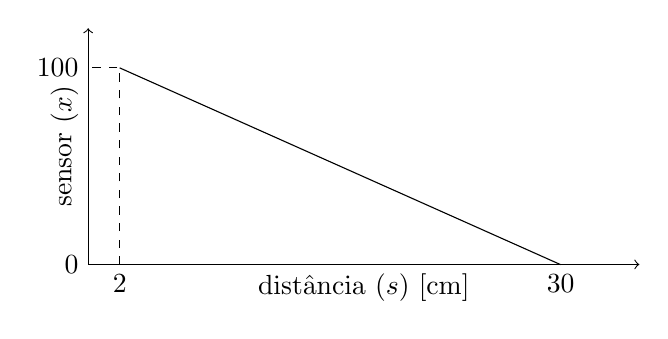
\begin{tikzpicture}
\draw[<->] (0,3) -- node[sloped,above,rotate=180] {\p{sensor ($x$)}} (0,0) node[left] {\p{0}} -- node[below] {\p{distância ($s$) [cm]}} (7,0);
\draw[dashed] (.4,0) node[below] {\p{2}} -- (.4,2.5) -- (0,2.5) node[left] {\p{100}};
\draw[domain=2:30] plot (\x/5,{(-3.57*\x+107)/40}) node[below] {\p{30}};
\end{tikzpicture}
\caption{Valor retornado como uma função linear da distância}\label{fig.linear}
\end{center}
\end{figure}

Vamos computar a inclinação e a interceptação:
\[
\textit{inclinação} = \frac{\Delta x}{\Delta s} = \frac{0-100}{30-2}=-3,\!57\,,
\]
onde $s=30$, $x=0=-3,\!57\cdot 30+b$, então $b=107$ e $x = -3,\!57 s + 107$. Resolver para $s$ dá uma função que o computador do robô pode usar para mapear um valor do sensor para a distância correspondente:
\[
s = \frac{107-x}{3,\!57}\,.
\]

\begin{framed}
\act{Linearidade}{linearity}
\begin{itemize}
\item Fixe uma régua em sua mesa e coloque cuidadosamente o robô de modo que seu sensor frontal seja posicionado ao lado da marca de $0$ da régua. Coloque um objeto ao lado da marca de $1$ cm na régua. Registre o valor retornado pelo sensor. Repita para distâncias de $2$ cm, $3$ cm, \ldots, até que o valor retornado vá para zero.
\item Plote um gráfico do valor retornado em função da distância. A resposta do sensor é linear? Em caso afirmativo, calcule a inclinação e a interceptação.
\item Repita o experimento com objetos de diferentes formas e materiais. A linearidade do gráfico depende das características do objeto?
\end{itemize}
\end{framed}

\subsection{Mapeamento de Sensores Não-lineares}

A Figura~\ref{fig.nonlinear} mostra um possível resultado das medições em Activity~\ref{act.linearity}. As medidas são mostradas como pontos junto com a função linear da Fig.~\ref{fig.linear}. A função é razoavelmente linear no meio de sua faixa, mas não-linear fora dessa faixa. Isto significa que é impossível usar uma função linear dos valores brutos do sensor para obter a distância de um objeto do robô.

\begin{figure}
\begin{center}
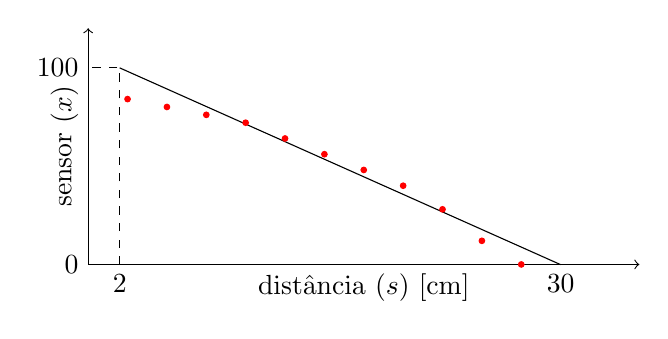
\begin{tikzpicture}
\draw[<->] (0,3) -- node[sloped,above,rotate=180] {\p{sensor ($x$)}} (0,0) node[left] {\p{0}} -- node[below] {\p{distância ($s$) [cm]}} (7,0);
\draw[dashed] (.4,0) node[below] {\p{2}} -- (.4,2.5) -- (0,2.5) node[left] {\p{100}};
\draw[domain=2:30] plot (\x/5,{(-3.57*\x+107)/40}) node[below] {\p{30}};
\foreach \x/\y in {0.5/2.5, 1/2.4, 1.5/2.3, 2/2.2, 2.5/2, 3/1.8, 3.5/1.6, 4/1.4, 4.5/1.1, 5/0.7, 5.5/0.4}
  \draw[fill,red,yshift=-4mm] (\x,\y) circle[radius=1pt];
\end{tikzpicture}
\caption{Valores experimentais retornados em função da distância}\label{fig.nonlinear}
\end{center}
\end{figure}

Podemos construir uma tabela para mapear os valores do sensor a distâncias. A tabela~\ref{tab.nonlinear} é uma tabela baseada em medições reais com um robô educacional. As medições foram feitas a cada dois centímetros, de $2$ cm a $18$ cm; a $20$ cm o sensor não detectou mais o objeto. A segunda coluna mostra o valor do sensor para cada distância. A terceira coluna mostra os valores $x_l$ que seriam devolvidos pelo sensor se ele fosse linear com a função $x=-2s+48$. Vemos que os valores reais retornados pelo sensor não se desviam muito da linearidade, portanto, pode ser razoável usar uma função linear.

\begin{table}
\begin{displaymath}
\begin{array}{r@{\hspace{2em}}r@{\hspace{2em}}r}
\hline\noalign{\smallskip}
s \textrm{(cm)} & x & x_l\\
%\multicolumn{1}{c}{s \textrm{(cm)}} & \multicolumn{1}{c}{x}& \multicolumn{1}{c}{x_l}\\
\noalign{\smallskip}\hline\noalign{\smallskip}
18 &14 & 12\\
16 &18 & 16\\
 14&22 & 20\\
 12&26 & 24\\
 10&29 & 28\\
 8 &32 & 32\\
 6 &36 & 36\\
 4 &41 & 40\\
 2 &44 & 44\\
\noalign{\smallskip}\hline\noalign{\smallskip}
\end{array}
\end{displaymath}
\caption{Mapeamento dos valores do sensor para distâncias}\label{tab.nonlinear}
\end{table}
Obviamente, seria melhor se tivéssemos uma entrada em tabela para cada um dos valores possíveis devolvidos pelo sensor. Entretanto, isto exigiria muita memória e pode ser impraticável se a faixa de valores retornados pelo sensor for muito maior, digamos, de $0$ a $4095$ ($12$ bits). Uma solução é pegar o valor mais próximo, de modo que se o valor $27$ for retornado pelo sensor cujo mapeamento é dado na Tabela~\ref{tab.nonlinear}, a distância indicada seria de $12$ cm.

Uma solução melhor é usar interpolação. Se você olhar novamente para o gráfico na Fig.~\ref{fig.nonlinear}, você pode ver que os segmentos da curva são mais ou menos lineares, embora suas inclinações mudem de acordo com a curva. Portanto, podemos obter uma boa aproximação da distância correspondente a um valor do sensor tomando a distância relativa em uma linha reta entre dois pontos (Fig.~\ref{fig.interpolation}). Dadas as distâncias $s_1$ e $s_2$ correspondentes aos valores do sensor $x_1$ e $x_2$, respectivamente, para um valor $x_1<x<x_2$, sua distância $s$:
\[
s = s_1 + \frac{s_2-s_1}{x_2-x_1}(x-x_1)\,.
\]

\begin{figure}
\begin{center}
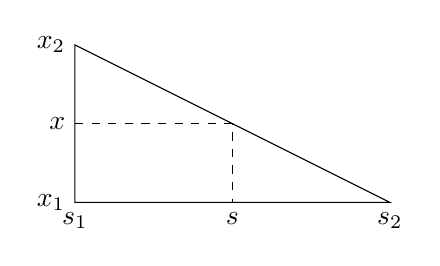
\begin{tikzpicture}
\draw (0,0) node[left] {$x_1$} -- (0,2) node[left] {$x_2$} -- (4,0) node[below] {$s_2$} -- cycle node[below] {$s_1$};
\draw[dashed] (0,1) node[left] {$x$} -| (2,1) -- (2,0) node[below] {$s$};
\end{tikzpicture}
\caption{Interpolação dos valores dos sensores}\label{fig.interpolation}
\end{center}
\end{figure}

\section{Sumário}

Ao projetar um robô, a escolha dos sensores é crítica. O projetista precisa decidir o que precisa para as medidas: distância, atitude, velocidade, etc. Então o projetista tem que fazer concessões: maior alcance, resolução, precisão e exatidão são sempre melhores, mas vêm com um preço. Para robôs educacionais, o preço é a consideração primordial, portanto não espere um bom desempenho de seu robô. No entanto, os princípios algorítmicos são os mesmos, quer os sensores sejam de alta qualidade ou não, portanto o compromisso não afeta a capacidade de aprender com o robô.

Qualquer sensor conectado ao computador do robô vai retornar valores discretos dentro de uma faixa fixa. O computador deve ser capaz de mapear tais valores para quantidades físicas em um processo chamado calibração. Se o sensor for linear, a calibração resulta em dois valores (inclinação e interceptação) que determinam uma função linear. Se o sensor for não-linear, uma tabela ou uma função não-linear deve ser usada.


\section{Outras leituras}

Para uma visão geral dos sensores usados em robôs móveis veja \cite[seção 4.1]{siegwart}. O livro de Everett \cite{everett} é inteiramente dedicado a este tópico.
